\newcommand{\VisParseSteps}{519}\newcommand{\VisParseMaxDepth}{24}
\newcommand{\VisOpSyms}{ADD,SUB,RET,CALL,LT,JZ,PUSH,STORE,LOAD}
\newcommand{\VisOpCoords}{(332,ADD) (464,SUB) (465,RET) (466,CALL) (531,LT) (531,JZ) (1027,PUSH) (1978,STORE) (3285,LOAD)}
\newcommand{\VisOpTotal}{9147}
\newcommand{\VisOpShare}{69}
\newcommand{\VisRounds}{6}\newcommand{\VisRewrites}{49}\newcommand{\VisRoundXTicks}{1,2,3,4,5,6}
\newcommand{\VisRaK}{4}\newcommand{\VisRaColors}{4}\newcommand{\VisRaSpills}{1}\newcommand{\VisRaMinK}{5}\newcommand{\VisRaVars}{8}
\newcommand{\VisSqlScanned}{8}\newcommand{\VisSqlPairs}{3}\newcommand{\VisSqlOps}{9}

\chapter{Visualisation}
\label{ch:vis}

\section{Why visualise a compiler?}
A compiler is invisible by nature: text goes in, text (or a number on the screen) comes out, and everything interesting happens in between. The studio exists to make the in-between visible. Students, reviewers and the author himself can \emph{see} the token stream, watch a parser stack grow and shrink, follow a loop through a control-flow graph, replay an optimizer's decisions, and compare a query plan before and after rewriting.

\begin{plain}
Reading about ``shift/reduce parsing'' is abstract; watching a stack of states fill up, one step at a time, with the reason for every action written next to it, makes it concrete. Every visualisation in this project follows that idea: \emph{show the real intermediate data, in a form a person can step through.}
\end{plain}

\section{Design principles}
\begin{enumerate}
  \item \textbf{Real data only.} Every view is rendered from the compiler's JSON. There is no mock data and no hand-drawn diagram of a ``typical'' run: if the compiler changes, the picture changes. (The data-driven figures in Section~\ref{sec:visfig} of this chapter and the page in the studio are generated the same way, by a script that runs the compiler.)
  \item \textbf{Time is a slider.} Anything that unfolds over time --- parsing, data-flow iteration, the VM, the debugger --- is recorded once and \emph{replayed}: first/previous/play/next/last controls and a scrubber. Replay makes backward stepping free and makes every state reproducible.
  \item \textbf{Linked views.} Selecting something in one view highlights it in another: a CFG block highlights its source lines; a token highlights its position in the source; a plan operator shows its measured row count.
  \item \textbf{Explain every step.} Wherever a step is shown, a sentence says \emph{why} it happened (``Lookahead \texttt{fn} is valid in state 0: push it and go to state 4'').
  \item \textbf{Consistent colour semantics.} The same colour always means the same thing (Table~\ref{tab:colours}).
  \item \textbf{Progressive disclosure.} Summary first (counts, chips), detail on demand (tabs, expandable plans, ``plan as written'').
\end{enumerate}

\begin{table}[H]\centering\small
\begin{tabular}{@{}lll@{}}\toprule
\textbf{Colour} & \textbf{Meaning} & \textbf{Where}\\ \midrule
\textcolor{teal}{\rule{8pt}{8pt}} green & success, ``true'' branch, verified fix, scan & status chips, CFG edges, assistant, SQL \code{Scan}\\
\textcolor{crimson}{\rule{8pt}{8pt}} red & error, ``false'' branch, unreachable block, stack-memory operand & diagnostics, CFG, native page\\
\textcolor{nova}{\rule{8pt}{8pt}} blue / violet & the focus: selection, registers, current step, join & selection, instruction pointer, SQL \code{Join}\\
\textcolor{amber}{\rule{8pt}{8pt}} amber & caution, jump, filter, back edge & warnings, CFG jump edges, SQL \code{Filter}\\ \bottomrule
\end{tabular}
\caption{Colour semantics used across the studio.}\label{tab:colours}
\end{table}

\section{Catalogue of visualisations}
\begin{table}[H]\centering\small
\begin{tabularx}{\textwidth}{@{}p{0.22\textwidth}p{0.27\textwidth}p{0.20\textwidth}X@{}}\toprule
\textbf{View} & \textbf{What it shows} & \textbf{Data source} & \textbf{Technique}\\ \midrule
Token table & every token with category, lexeme, terminal, line:column & \code{tokens} & table; selection highlights source range\\
Parse trace & LR(1) stack, remaining input, action and its explanation per step & \code{parser.trace} & replayable stepper, scrubber, play/pause\\
FIRST/FOLLOW, LR(1) states & grammar sets; kernel and closure items per state & \code{/api/grammar} & lazy-loaded tables\\
Parse tree, AST & concrete and abstract syntax trees & \code{parser.tree}, \code{ast} & React Flow graph with a custom tidy-tree layout\\
Symbol tables & scopes, symbols, types, read/write sites & \code{semantic} & nested scope tree\\
IR & instructions before/after optimization with explanations & \code{ir} & aligned listings\\
CFG & blocks, labelled edges, back edges, dominators, unreachable blocks & \code{analysis.blocks/edges} & React Flow with a layered layout; edge colours by kind\\
Data-flow & USE/DEF/IN/OUT per block per iteration & \code{liveness}, \code{reachingDefinitions} & stepper over \code{history}; changed sets highlighted\\
SSA & $\varphi$ placement and renamed code per block & \code{ssa} & per-block listing\\
Optimization history & each rewrite: pass, before $\to$ after, reason & \code{optimization.history} & filterable table; per-pass impact table\\
Bytecode, VM state & instruction listing; frames, locals, operand stack & \code{bytecode}, trace snapshots & listing with current-instruction marker; stack diagram\\
Debugger & source, breakpoints, call stack, output & \code{/api/debug/*} & Monaco decorations + replay\\
Native x86-64 & assembly, registers vs.\ stack slots, memory-operand count & \code{/api/asm} & token-level syntax colouring, comparison bars\\
SQL plan & operator tree with measured rows & \code{plan.tree} & indented tree with proportional bars\\
SQL rewrites & rule, explanation, plan before/after & \code{plan.history} & side-by-side text\\
Assistant diffs & unified diff of each fix & \code{/api/suggest} & coloured diff, verified badge\\ \bottomrule
\end{tabularx}
\caption{Every visualisation, its data source and technique.}
\end{table}

\section{A gallery}
Figure~\ref{fig:gallery} shows four of the views side by side; each is a full-size screenshot elsewhere in the report (Chapters~\ref{ch:backends}, \ref{ch:sql} and~\ref{ch:platform}).

\begin{figure}[H]\centering
\begin{subfigure}[b]{0.49\textwidth}\fbox{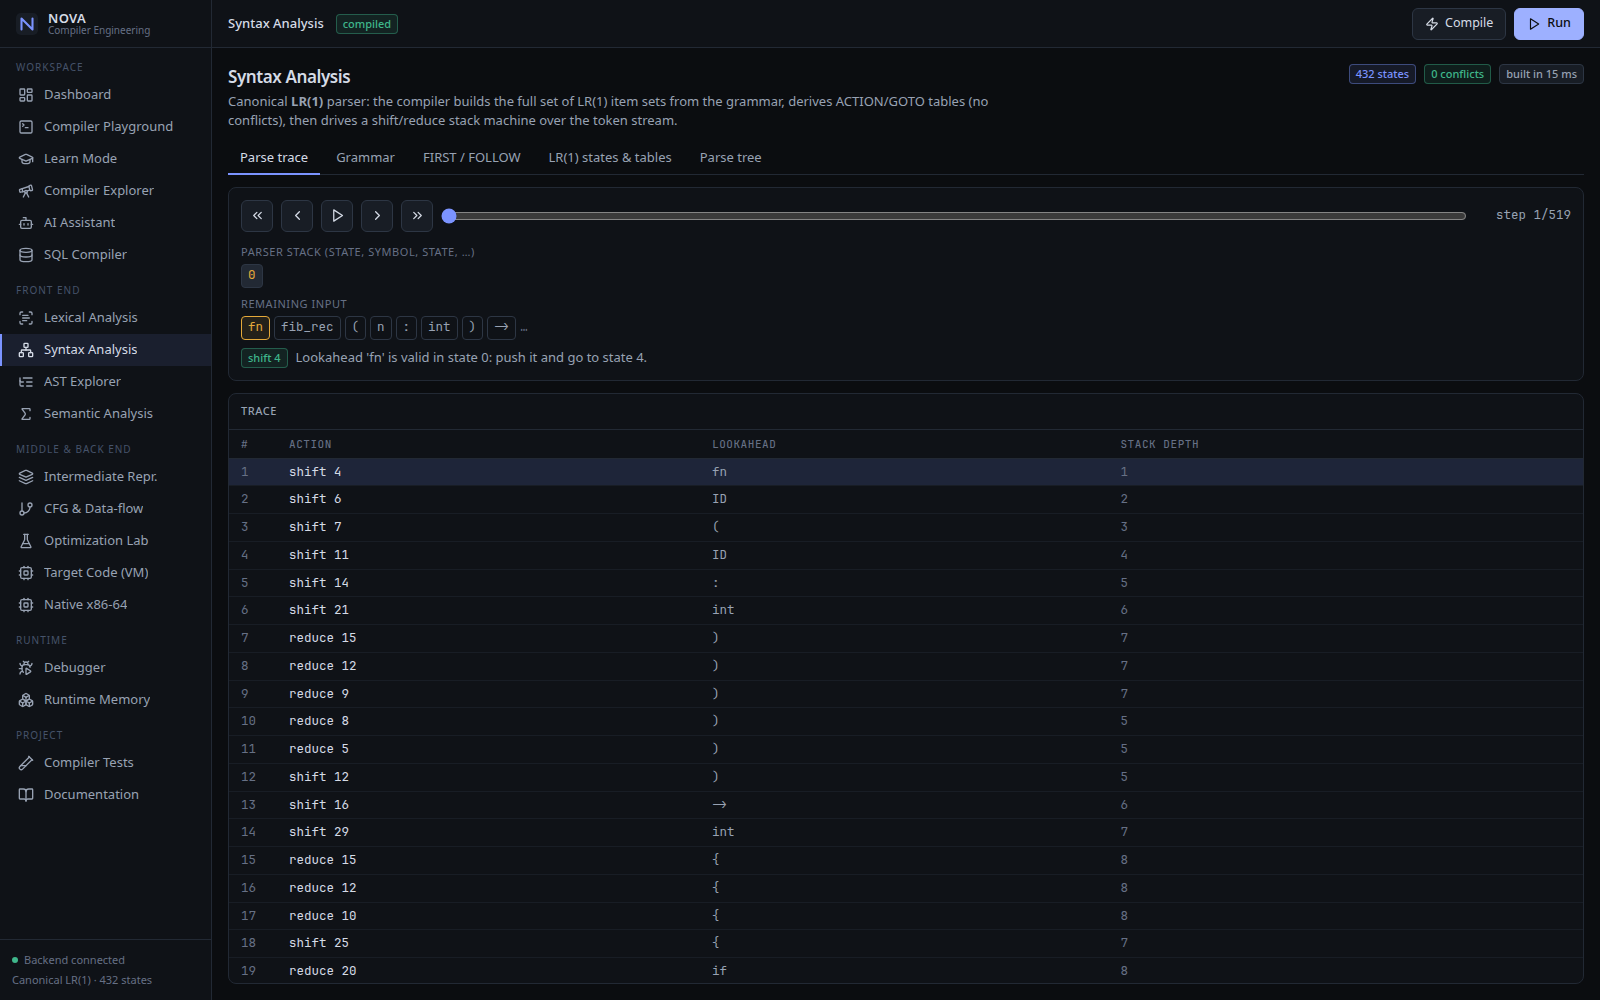
\includegraphics[width=\textwidth]{img/ui_syntax.png}}\caption{LR(1) parse trace}\end{subfigure}\hfill
\begin{subfigure}[b]{0.49\textwidth}\fbox{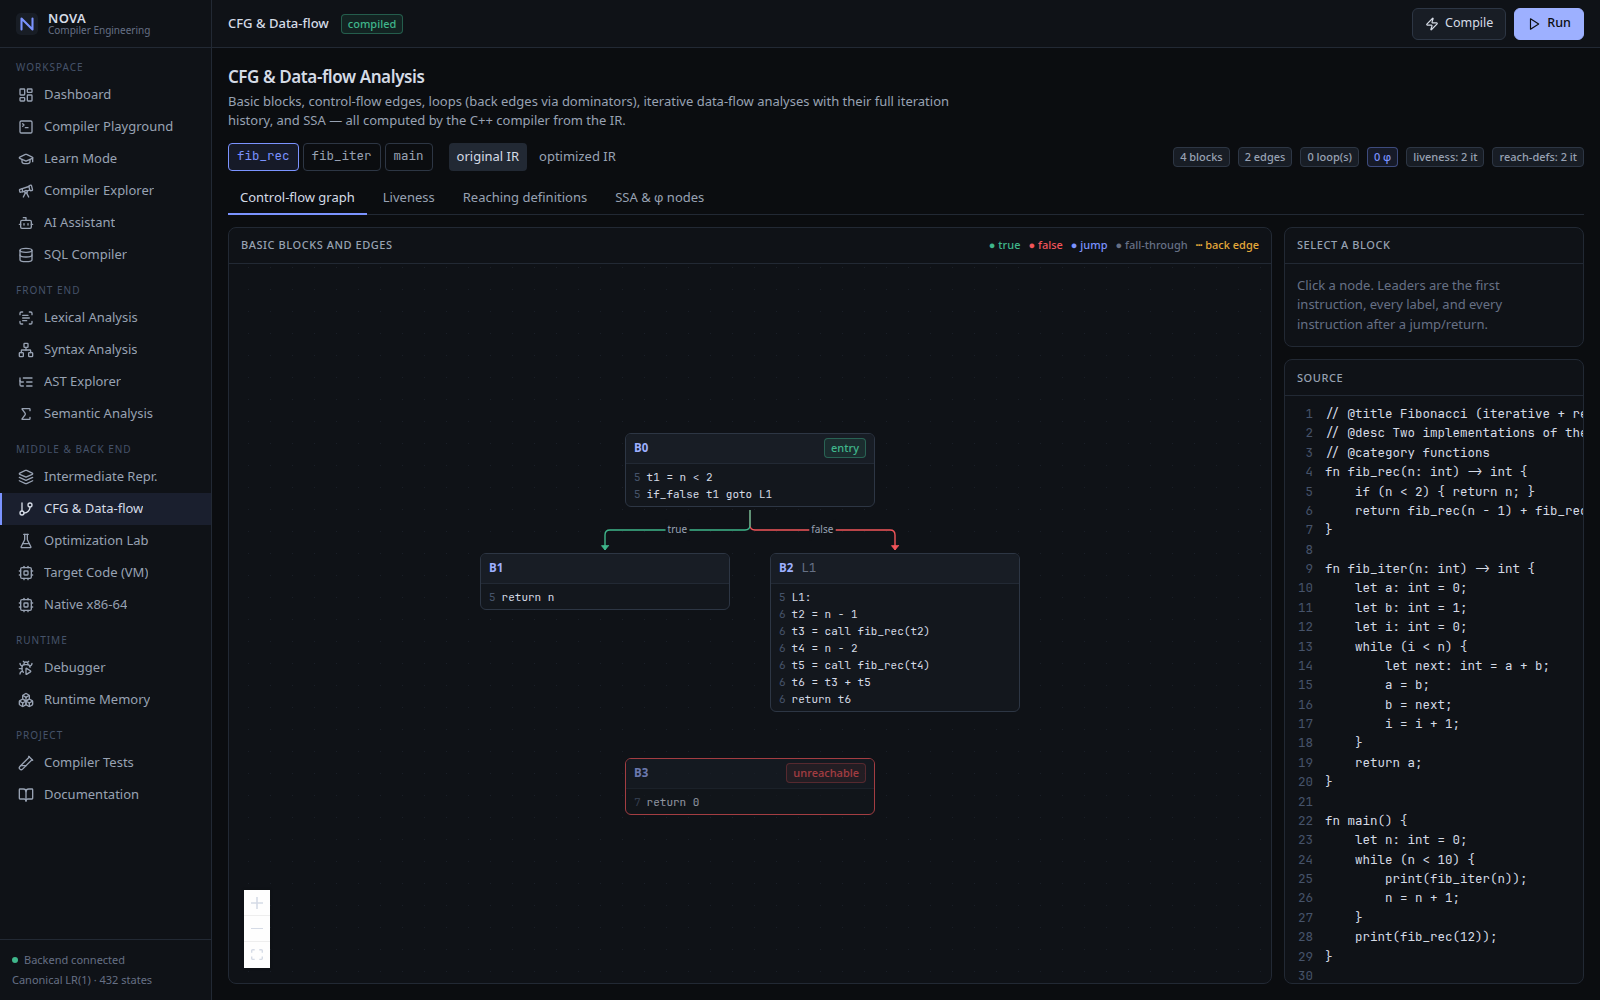
\includegraphics[width=\textwidth]{img/ui_analysis.png}}\caption{CFG with true/false edges}\end{subfigure}\\[6pt]
\begin{subfigure}[b]{0.49\textwidth}\fbox{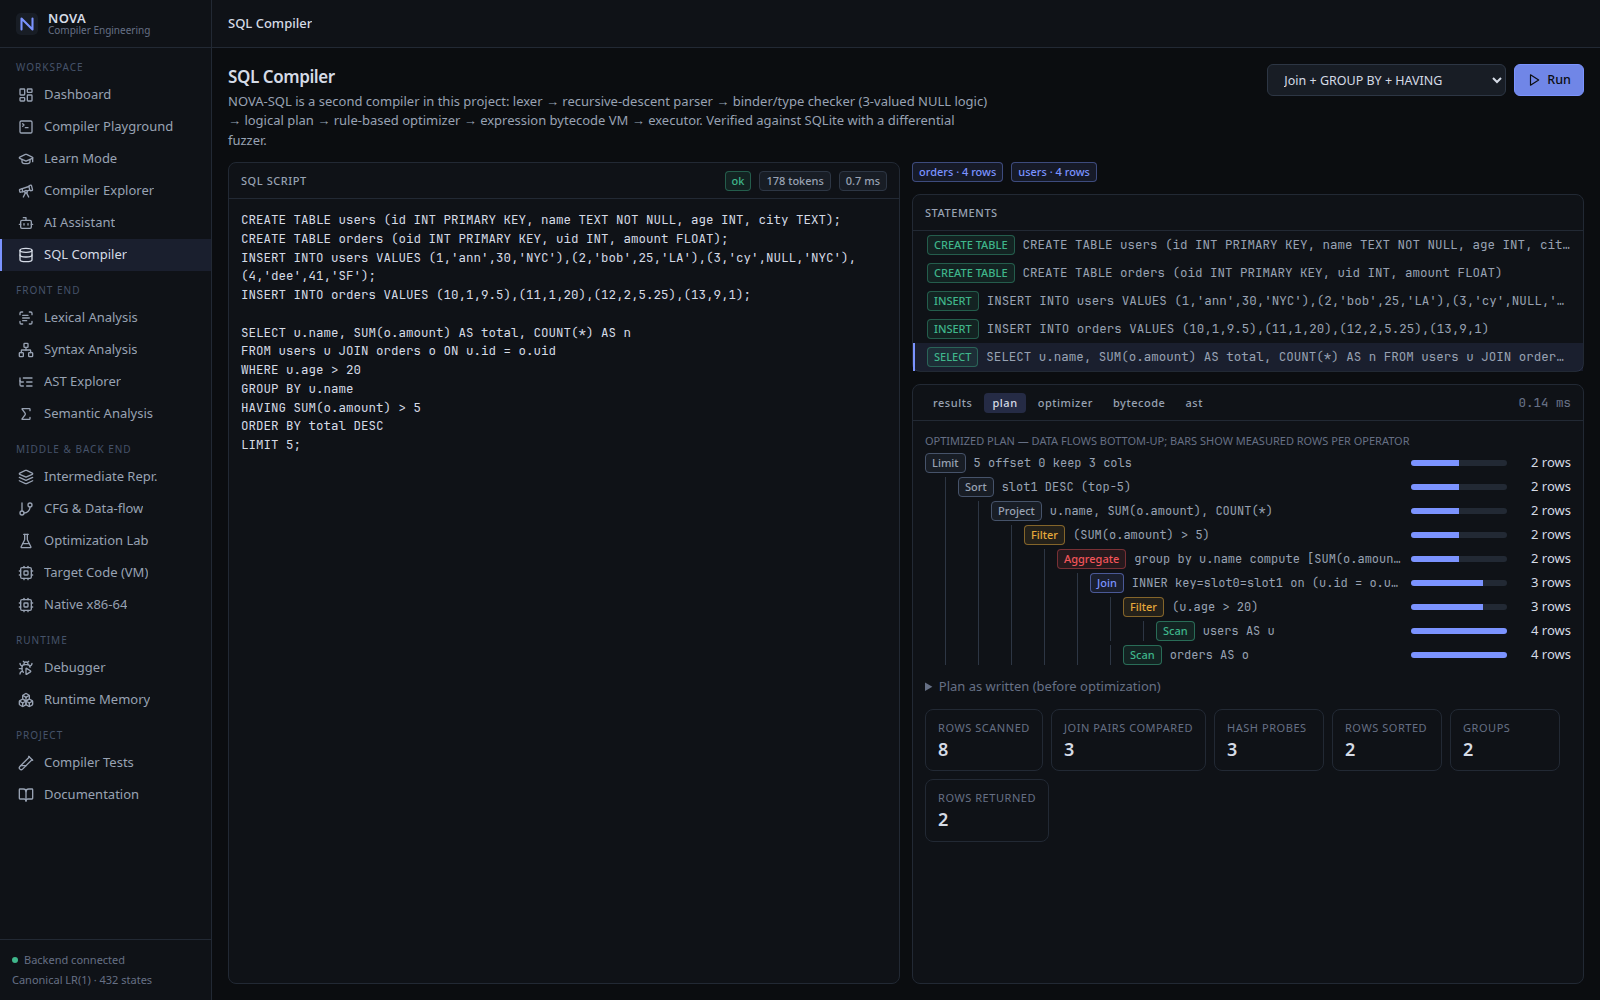
\includegraphics[width=\textwidth]{img/ui_sql_plan.png}}\caption{SQL plan with measured rows}\end{subfigure}\hfill
\begin{subfigure}[b]{0.49\textwidth}\fbox{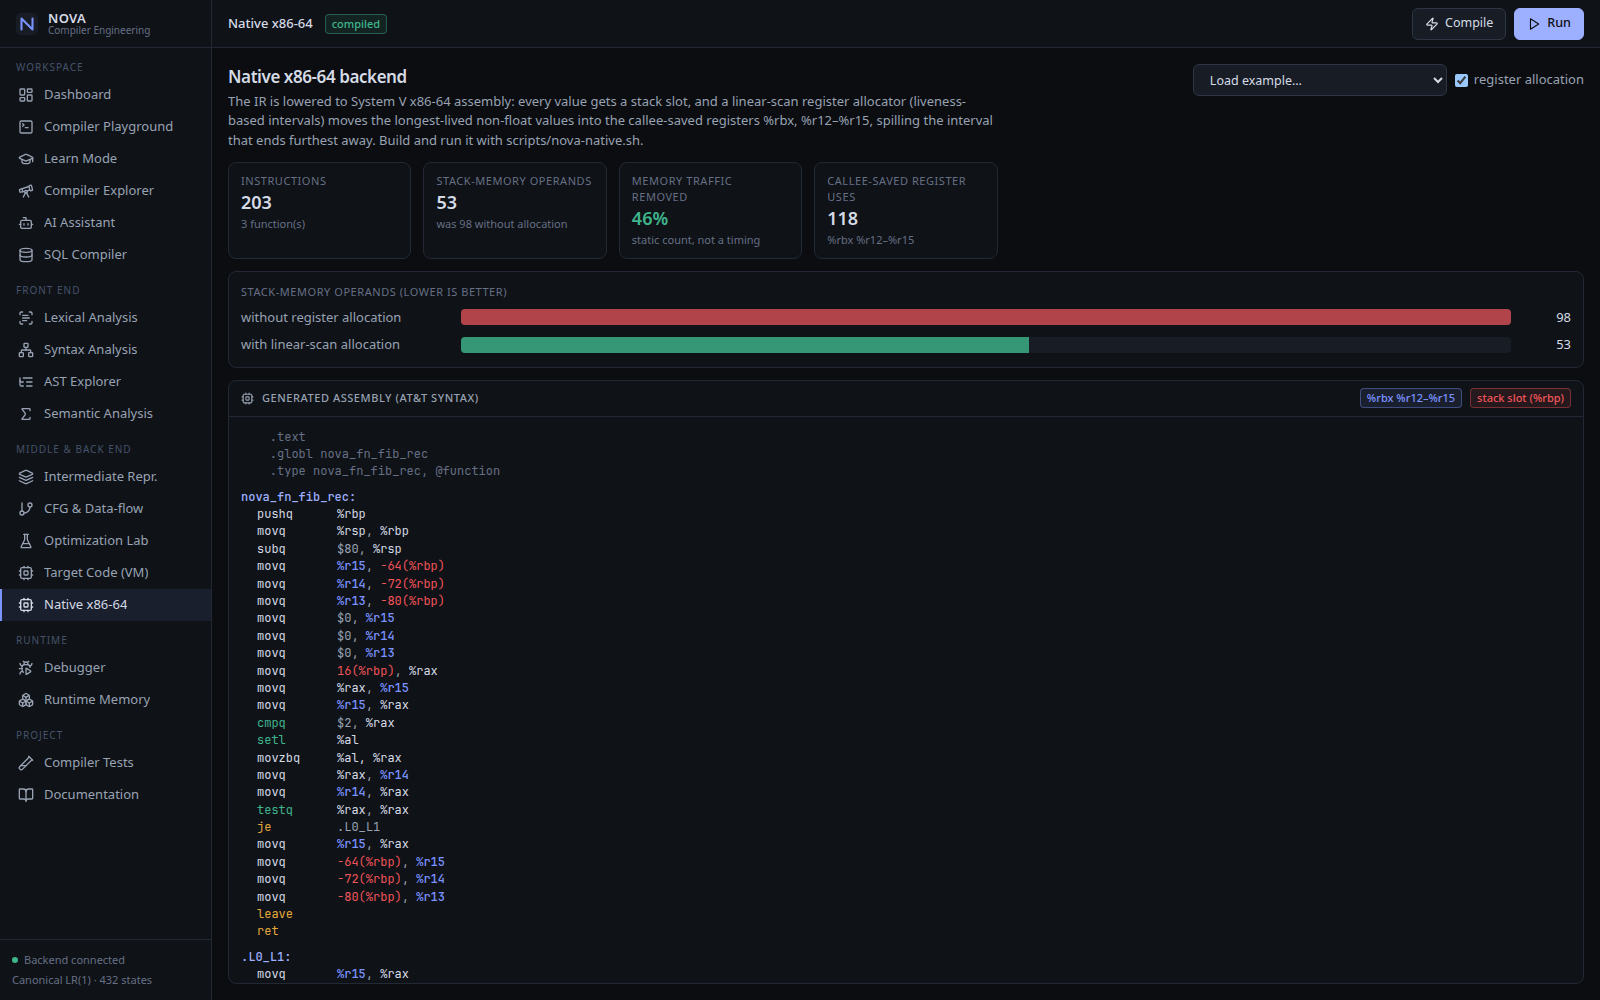
\includegraphics[width=\textwidth]{img/ui_native.png}}\caption{Native code and register use}\end{subfigure}
\caption{Four of the studio's views.}\label{fig:gallery}
\end{figure}

\section{The Visualisation page}
The studio has a dedicated \textbf{Visualisation} page (left menu, \emph{Workspace} group) that brings the data-driven charts together for \emph{whatever program is currently in the Playground}: parser stack depth, a VM instruction histogram (press \emph{Run to collect VM stats}), optimizer rewrites per round and pass, live ranges coloured by register (one tab per function), and the measured row counts of an optimized SQL plan, with links to the detailed views.

\shot{ui_visualisation}{The studio's Visualisation page for the Fibonacci example (live data, no mock values).}

\section{Figures computed from real compiler data}\label{sec:visfig}
The five figures below reproduce, for the report, the same kind of charts: a script (\code{report/tools/gen\_vis.py}) runs the compiler on shipped examples and emits the plot data. They show the kind of insight the data makes visible.

\subsection{How the LR(1) parser stack grows}
Figure~\ref{fig:parsedepth} plots the parser stack depth at every step of parsing the shipped example \texttt{03\_fibonacci} (\VisParseSteps{} steps). The stack deepens as the parser enters nested constructs (a function, a block, an expression) and unwinds as it reduces them; its maximum of \VisParseMaxDepth{} is the deepest nesting, here a call inside an expression inside a \code{while} body.

\begin{figure}[H]\centering
\begin{tikzpicture}
\begin{axis}[width=0.92\textwidth,height=5.2cm,xlabel={parse step},ylabel={stack depth (symbols)},font=\sffamily\small,axis x line*=bottom,axis y line*=left,xmin=0,ymin=0,grid=major,grid style={dotted,grey!50}]
\addplot[nova,thick,const plot] coordinates {(1,1) (4,4) (7,7) (10,5) (13,6) (16,8) (19,8) (22,11) (25,12) (28,12) (31,14) (34,14) (37,12) (40,12) (43,14) (46,17) (49,17) (52,17) (55,17) (58,18) (61,15) (64,15) (67,9) (70,12) (73,13) (76,13) (79,15) (82,15) (85,13) (88,13) (91,14) (94,11) (97,11) (100,14) (103,15) (106,15) (109,17) (112,17) (115,15) (118,15) (121,16) (124,13) (127,11) (130,11) (133,11) (136,10) (139,8) (142,3) (145,6) (148,8) (151,6) (154,8) (157,9) (160,10) (163,13) (166,14) (169,16) (172,16) (175,16) (178,16) (181,11) (184,12) (187,14) (190,16) (193,16) (196,16) (199,16) (202,11) (205,11) (208,14) (211,15) (214,16) (217,16) (220,16) (223,17) (226,10) (229,13) (232,13) (235,13) (238,15) (241,15) (244,13) (247,13) (250,16) (253,19) (256,20) (259,22) (262,22) (265,24) (268,24) (271,22) (274,22) (277,17) (280,17) (283,19) (286,19) (289,19) (292,19) (295,17) (298,18) (301,19) (304,19) (307,19) (310,20) (313,16) (316,19) (319,19) (322,20) (325,21) (328,19) (331,19) (334,20) (337,16) (340,11) (343,11) (346,12) (349,12) (352,12) (355,12) (358,11) (361,9) (364,3) (367,6) (370,9) (373,12) (376,14) (379,16) (382,16) (385,16) (388,16) (391,11) (394,11) (397,13) (400,13) (403,14) (406,15) (409,15) (412,13) (415,14) (418,17) (421,20) (424,21) (427,21) (430,21) (433,21) (436,19) (439,19) (442,19) (445,19) (448,21) (451,16) (454,19) (457,19) (460,20) (463,21) (466,19) (469,19) (472,20) (475,16) (478,11) (481,11) (484,14) (487,15) (490,15) (493,15) (496,15) (499,13) (502,13) (505,13) (508,13) (511,15) (514,10) (517,3) (519,2)};
\end{axis}
\end{tikzpicture}

\caption{Parser stack depth over the \VisParseSteps{} steps of parsing \texttt{03\_fibonacci}.}\label{fig:parsedepth}
\end{figure}

\subsection{What the VM actually executes}
Figure~\ref{fig:opcodes} counts the instructions the optimized program executed. \VisOpShare{}\% of the \VisOpTotal{} executed instructions are \code{LOAD}, \code{STORE} or \code{PUSH}: a stack machine spends most of its time moving values around, not computing. This is the empirical motivation for the native back end and for register allocation (Chapter~\ref{ch:backends}), where those moves largely disappear.

\begin{figure}[H]\centering
\begin{tikzpicture}
\begin{axis}[xbar,width=0.85\textwidth,height=6.2cm,bar width=9pt,xmin=0,xmax=4000,symbolic y coords={ADD,SUB,RET,CALL,LT,JZ,PUSH,STORE,LOAD},ytick=data,nodes near coords,axis x line*=bottom,axis y line*=left,xlabel={times executed},font=\sffamily\small,enlarge y limits=0.08]
\addplot[fill=nova!75,draw=none] coordinates {(332,ADD) (464,SUB) (465,RET) (466,CALL) (531,LT) (531,JZ) (1027,PUSH) (1978,STORE) (3285,LOAD)};
\end{axis}
\end{tikzpicture}

\caption{VM instruction histogram for \texttt{03\_fibonacci} (optimized program).}\label{fig:opcodes}
\end{figure}

\subsection{How the optimizer converges}
Figure~\ref{fig:rounds} stacks the \VisRewrites{} rewrites the optimizer made on \texttt{04\_optimization\_demo} by round and pass. Round~1 does the most varied work (propagation, folding, algebra, CSE); round~2 mops up what that exposed (new constants to propagate, dead stores to delete); later rounds make single clean-up rewrites until the \emph{fixed point} is reached (a final round with no change then stops the loop). It is a direct picture of the pass manager's ``repeat until nothing changes'' design.

\begin{figure}[H]\centering
\begin{tikzpicture}
\begin{axis}[ybar stacked,width=0.9\textwidth,height=6cm,bar width=22pt,xlabel={optimization round},ylabel={rewrites},xtick={1,2,3,4,5,6},font=\sffamily\small,axis x line*=bottom,axis y line*=left,legend style={at={(1.02,0.5)},anchor=west,font=\sffamily\scriptsize},ymin=0,enlarge x limits=0.12]
\addplot[fill=nova!80,draw=none] coordinates {(1,5) (2,6) (3,1) (4,1) (5,1) (6,1)};
\addplot[fill=teal!80,draw=none] coordinates {(1,3) (2,1) (3,1) (4,1) (5,1) (6,0)};
\addplot[fill=amber!80,draw=none] coordinates {(1,6) (2,0) (3,0) (4,0) (5,0) (6,0)};
\addplot[fill=crimson!80,draw=none] coordinates {(1,1) (2,0) (3,0) (4,0) (5,0) (6,0)};
\addplot[fill=grey!80,draw=none] coordinates {(1,3) (2,0) (3,0) (4,0) (5,0) (6,0)};
\addplot[fill=novadark!80,draw=none] coordinates {(1,6) (2,7) (3,1) (4,1) (5,1) (6,1)};
\legend{constant propagation,constant folding,algebraic,cse,unreachable,dce}
\end{axis}
\end{tikzpicture}

\caption{Optimizer rewrites per round and pass on \texttt{04\_optimization\_demo}.}\label{fig:rounds}
\end{figure}

\subsection{Live ranges and register colours}
Figure~\ref{fig:intervals} draws the live range of every variable of \code{fib\_iter} from the liveness analysis, coloured by the graph-colouring allocator of the studio's \emph{CFG \& Data-flow} page with $K=\VisRaK$ registers: \VisRaVars{} variables, \VisRaColors{} colours used, \VisRaSpills{} spill, and \VisRaMinK{} registers needed for no spill at all. Two bars of the same colour never overlap in time --- that is precisely the condition for two variables to share a register.

\begin{figure}[H]\centering
\begin{tikzpicture}[x=1cm,y=1cm]
\node[anchor=east,font=\ttfamily\scriptsize] at (-0.15,0.0) {a};
\fill[crimson!75,rounded corners=1.5pt] (0.0,-0.2) rectangle (8.100000000000001,0.2);
\node[anchor=west,font=\sffamily\tiny,color=grey] at (8.250000000000002,0.0) {colour 3};
\node[anchor=east,font=\ttfamily\scriptsize] at (-0.15,-0.62) {n};
\fill[black!75,rounded corners=1.5pt] (0.0,-0.8200000000000001) rectangle (2.6,-0.42);
\node[anchor=west,font=\sffamily\tiny,color=grey] at (2.75,-0.62) {spilled};
\node[anchor=east,font=\ttfamily\scriptsize] at (-0.15,-1.24) {b};
\fill[amber!75,rounded corners=1.5pt] (0.55,-1.44) rectangle (5.3500000000000005,-1.04);
\node[anchor=west,font=\sffamily\tiny,color=grey] at (5.5,-1.24) {colour 2};
\node[anchor=east,font=\ttfamily\scriptsize] at (-0.15,-1.8599999999999999) {i};
\fill[teal!75,rounded corners=1.5pt] (1.1,-2.06) rectangle (6.450000000000001,-1.66);
\node[anchor=west,font=\sffamily\tiny,color=grey] at (6.6000000000000005,-1.8599999999999999) {colour 1};
\node[anchor=east,font=\ttfamily\scriptsize] at (-0.15,-2.48) {t1};
\fill[nova!75,rounded corners=1.5pt] (2.2,-2.68) rectangle (3.15,-2.28);
\node[anchor=west,font=\sffamily\tiny,color=grey] at (3.3,-2.48) {colour 0};
\node[anchor=east,font=\ttfamily\scriptsize] at (-0.15,-3.1) {t2};
\fill[nova!75,rounded corners=1.5pt] (3.3000000000000003,-3.3000000000000003) rectangle (4.250000000000001,-2.9);
\node[anchor=west,font=\sffamily\tiny,color=grey] at (4.4,-3.1) {colour 0};
\node[anchor=east,font=\ttfamily\scriptsize] at (-0.15,-3.7199999999999998) {next};
\fill[nova!75,rounded corners=1.5pt] (3.8500000000000005,-3.92) rectangle (5.3500000000000005,-3.5199999999999996);
\node[anchor=west,font=\sffamily\tiny,color=grey] at (5.5,-3.7199999999999998) {colour 0};
\node[anchor=east,font=\ttfamily\scriptsize] at (-0.15,-4.34) {t3};
\fill[nova!75,rounded corners=1.5pt] (5.5,-4.54) rectangle (6.450000000000001,-4.14);
\node[anchor=west,font=\sffamily\tiny,color=grey] at (6.6000000000000005,-4.34) {colour 0};
\draw[->,thick] (0,-4.76) -- (8.9,-4.76) node[right,font=\sffamily\scriptsize]{IR instruction index};

\end{tikzpicture}
\caption{Live ranges of the variables of \texttt{fib\_iter}, coloured by register assignment (black = spilled).}\label{fig:intervals}
\end{figure}

\subsection{Where a query's rows go}
Figure~\ref{fig:sqlrows} shows the measured row count at every operator of the optimized plan of the order-report query of Chapter~\ref{ch:sql} (data flows from the bottom to the top). The query scanned \VisSqlScanned{} rows in total; thanks to predicate pushdown and the hash join only \VisSqlPairs{} row pairs were compared in the join. The ``funnel'' shape --- many rows at the bottom, few at the top --- is what a good plan looks like.

\begin{figure}[H]\centering
\begin{tikzpicture}[x=1cm,y=1cm]
\node[anchor=west,font=\sffamily\scriptsize] at (0.0,0.0) {Limit};
\fill[nova!70,rounded corners=1pt] (4.6,-0.17) rectangle (6.3999999999999995,0.17);
\node[anchor=west,font=\sffamily\scriptsize] at (6.5,0.0) {2};
\node[anchor=west,font=\sffamily\scriptsize] at (0.3,-0.55) {Sort};
\fill[nova!70,rounded corners=1pt] (4.6,-0.7200000000000001) rectangle (6.3999999999999995,-0.38);
\node[anchor=west,font=\sffamily\scriptsize] at (6.5,-0.55) {2};
\node[anchor=west,font=\sffamily\scriptsize] at (0.6,-1.1) {Project};
\fill[nova!70,rounded corners=1pt] (4.6,-1.27) rectangle (6.3999999999999995,-0.93);
\node[anchor=west,font=\sffamily\scriptsize] at (6.5,-1.1) {2};
\node[anchor=west,font=\sffamily\scriptsize] at (0.8999999999999999,-1.6500000000000001) {Filter};
\fill[nova!70,rounded corners=1pt] (4.6,-1.82) rectangle (6.3999999999999995,-1.4800000000000002);
\node[anchor=west,font=\sffamily\scriptsize] at (6.5,-1.6500000000000001) {2};
\node[anchor=west,font=\sffamily\scriptsize] at (1.2,-2.2) {Aggregate};
\fill[nova!70,rounded corners=1pt] (4.6,-2.37) rectangle (6.3999999999999995,-2.0300000000000002);
\node[anchor=west,font=\sffamily\scriptsize] at (6.5,-2.2) {2};
\node[anchor=west,font=\sffamily\scriptsize] at (1.5,-2.75) {Join};
\fill[nova!70,rounded corners=1pt] (4.6,-2.92) rectangle (7.3,-2.58);
\node[anchor=west,font=\sffamily\scriptsize] at (7.4,-2.75) {3};
\node[anchor=west,font=\sffamily\scriptsize] at (1.7999999999999998,-3.3000000000000003) {Filter};
\fill[nova!70,rounded corners=1pt] (4.6,-3.47) rectangle (7.3,-3.1300000000000003);
\node[anchor=west,font=\sffamily\scriptsize] at (7.4,-3.3000000000000003) {3};
\node[anchor=west,font=\sffamily\scriptsize] at (2.1,-3.8500000000000005) {Scan};
\fill[nova!70,rounded corners=1pt] (4.6,-4.0200000000000005) rectangle (8.2,-3.6800000000000006);
\node[anchor=west,font=\sffamily\scriptsize] at (8.3,-3.8500000000000005) {4};
\node[anchor=west,font=\sffamily\scriptsize] at (1.7999999999999998,-4.4) {Scan};
\fill[nova!70,rounded corners=1pt] (4.6,-4.57) rectangle (8.2,-4.23);
\node[anchor=west,font=\sffamily\scriptsize] at (8.3,-4.4) {4};

\end{tikzpicture}
\caption{Rows produced by each operator of the optimized plan (top = last operator, bottom = scans; indentation shows nesting).}\label{fig:sqlrows}
\end{figure}

\section{Implementation notes}
\begin{itemize}
  \item \textbf{Graphs.} AST and CFG views use React Flow with layout algorithms written for this project (tidy tree for the AST, layered layout with back-edge routing for the CFG). The layouts are pure functions and are covered by unit tests (\code{features/ast/layout.test.ts}, \code{features/cfg/layout.test.ts}).
  \item \textbf{Editor.} Monaco provides diagnostics squiggles from compiler ranges, breakpoints and current-line decoration in the debugger, and a custom \nova{} syntax definition (keywords, types, built-ins, strings).
  \item \textbf{Replay.} Parse traces, data-flow histories and VM snapshots are plain arrays; a shared stepper component moves an index over them, so the same controls work for all.
  \item \textbf{Plan tree.} A recursive component draws operators with an operator-coloured badge and a bar proportional to the measured rows relative to the largest operator.
  \item \textbf{Assembly colouring.} A small tokenizer colours mnemonics (jumps and calls amber, compares green), callee-saved registers blue and stack slots red, so register allocation is visible at a glance.
  \item \textbf{Lazy loading.} Pages and heavy components (Monaco, React Flow) are loaded on demand, so the first screen appears quickly.
\end{itemize}

\section{How the visualisations were checked}
Each page was loaded in a headless Chrome driven by Playwright, example programs were selected, buttons clicked, and the console watched: \textbf{zero browser errors} over the whole tour; the screenshots in this report come from that run. Vitest tests cover the layout algorithms, the data-flow stepper, the SQL page (rows, NULL rendering, optimizer history, API failure) and the assistant page (verified badges, diffs, inline code, ``not configured'' state).

\begin{warnbox}
Not verified: accessibility (screen-reader support, colour-blind palettes beyond the use of labels and icons alongside colour), narrow-screen layouts beyond the responsive breakpoints in the CSS, and the layout of very large graphs (hundreds of basic blocks).
\end{warnbox}
